\documentclass{article}
\usepackage[T1]{fontenc}
\usepackage{lmodern}
\usepackage{graphicx}
\usepackage{amsmath,amssymb}
\usepackage[a4paper,margin=2cm]{geometry}
\usepackage[absolute,overlay]{textpos}
\setlength{\TPHorizModule}{1mm}
\setlength{\TPVertModule}{1mm}
\usepackage[indonesian]{babel}
\usepackage{hyperref}
\setlength{\emergencystretch}{2em}
% unit: Halaman 39

\begin{document}

% === Halaman 39 (llm) ===

\vspace{172.26mm}

\section*{Electromagnetic eavesdropping}

\vspace{50mm}

Sumber: \url{https://www.researchgate.net/figure/An-anechoic-chamber-Figure-4-Example-for-an-electromagnetic-eavesdropping-process_fig3_324680618}

% deskripsi: Ilustrasi konsep eavesdropping elektromagnetik yang menunjukkan seseorang di satu kantor menggunakan antena penerima untuk menangkap sinyal dari perangkat elektronik (komputer) di kantor sebelah melalui dinding, dengan keterangan jarak r < 2m.
% bbox normalisasi: [0.1300, 0.1600, 0.7800, 0.7400]
\begin{textblock*}{136.50mm}(27.30mm,47.52mm)
\noindent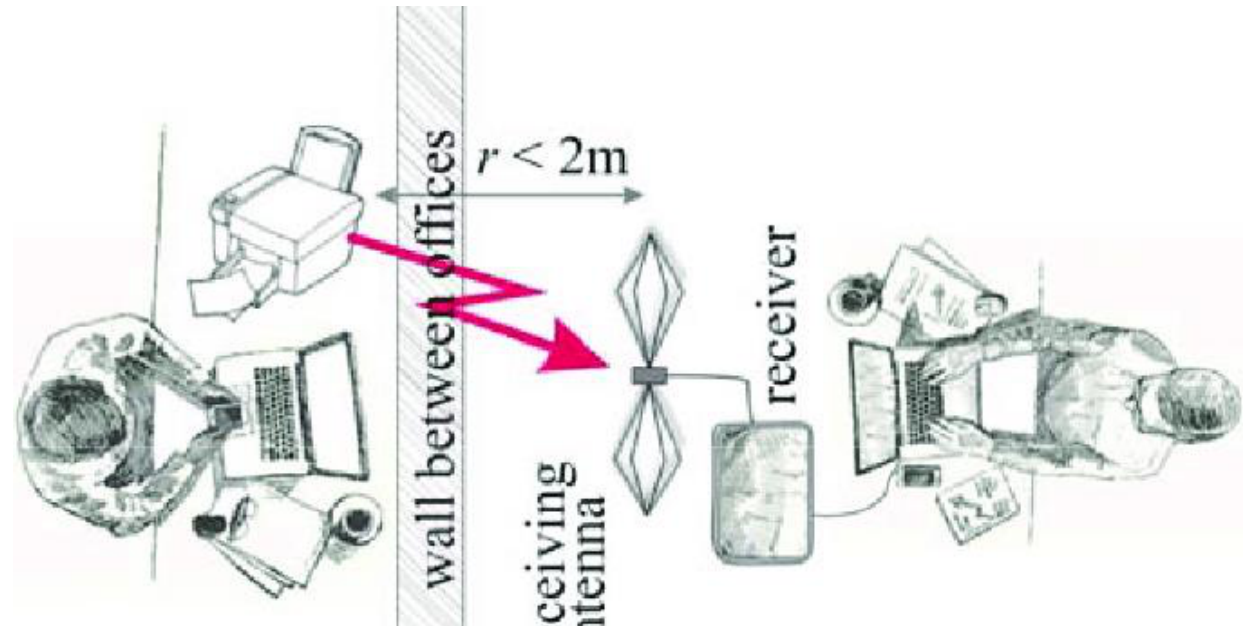
\includegraphics[width=136.50mm,height=172.26mm]{../../images/llm/page_039_img_01.png}%
\end{textblock*}

\end{document}
